\PassOptionsToPackage{table, dvipsnames}{xcolor}

\documentclass[a4paper,twoside,12pt]{toptesi}

%-------------------------------------------------------------------------------
% CONFIGURAZIONE BASE DEL DOCUMENTO
%-------------------------------------------------------------------------------
\usepackage[T1]{fontenc}
\usepackage[utf8]{inputenc}
\usepackage[italian]{babel}
\usepackage{amssymb}
\usepackage{amsmath}

%-------------------------------------------------------------------------------
% PACKAGE PER GRAFICA E IMMAGINI
%-------------------------------------------------------------------------------
\usepackage{multirow}
\usepackage{geometry}
\geometry{a4paper, margin=1in}
\usepackage{graphicx}
\usepackage{tikz}
\usetikzlibrary{positioning}
\usepackage{listings}
\usepackage[font=small,skip=10pt]{caption}
\usepackage{subcaption}
\usepackage{booktabs} 
\usepackage{longtable} 
\usepackage{float} 
\usepackage{caption} 
\usepackage{siunitx} 
\usepackage{makecell}

%-------------------------------------------------------------------------------
% PACKAGE PER COLORI E TABELLE
%-------------------------------------------------------------------------------

\usepackage[table]{xcolor}
\usepackage{booktabs}

%-------------------------------------------------------------------------------
% PACKAGE PER CODICE SORGENTE
%-------------------------------------------------------------------------------
\usepackage{minted}
\usepackage{amssymb} % if not already loaded

\setminted{
  style=friendly,
  linenos=true,
  frame=lines,
  framesep=2mm,
  bgcolor=gray!10,
  fontsize=\small,
  autogobble=true,
  breaklines=true,
  breakanywhere=true,
  breakindent=15pt,
  breakautoindent=true,
  breaksymbolleft=\mbox{\tiny\color{red}{\ensuremath{\Lsh}}\space},
}

%-------------------------------------------------------------------------------
% PACKAGE PER MATEMATICA E UNITÀ DI MISURA
%-------------------------------------------------------------------------------
\usepackage{siunitx}

%-------------------------------------------------------------------------------
% PACKAGE PER LISTE
%-------------------------------------------------------------------------------
\usepackage{enumitem}

%-------------------------------------------------------------------------------
% PACKAGE PER IPERTESTI E RIFERIMENTI
%-------------------------------------------------------------------------------
\usepackage{hyperref}
\hypersetup{
    pdfkeywords={Malware Detection, Fourier-BERT, Machine Learning, Cybersecurity, NLP},
    colorlinks=true,
    linkcolor=black,
    citecolor=Green,
    urlcolor=NavyBlue,
    filecolor=magenta,
    bookmarksnumbered=true,
    breaklinks=true,
    pdfpagemode=UseOutlines,
    pdfstartview=FitH,
    unicode=true
}

%-------------------------------------------------------------------------------
% IMPOSTAZIONI DI FORMATTAZIONE
%-------------------------------------------------------------------------------
\linespread{1.25}

\let\savedlisting\listing% save original definition
\AtBeginDocument{\let\listing\savedlisting}

%-------------------------------------------------------------------------------
% DEFINIZIONI PER IL FRONTESPIZIO (MACRO PERSONALIZZATE DALLA CLASSE toptesi)
%-------------------------------------------------------------------------------
\def\dept{DIPARTIMENTO DI INFORMATICA}
\def\course{CORSO DI LAUREA IN INFORMATICA}

\def\title{Analisi dei Pattern delle Chiamate Api per la Classificazione Malware}
\def\author{Giacomo Gaudio}
\def\relatoreone{Prof.ssa Annalisa Appice}
\def\relatoretwo{Dr. Giuseppina Andresini}
\def\correlatoreone{}
\def\correlatoretwo{}
\def\subject{}
\def\annoacc{2024 \- 2025}
\def\beforecandidate{LAUREANDO:}
\def\beforetitle{TESI DI LAUREA \\ IN \\ }
\def\beforeprof{RELATORI:}
\def\beforecorrelatore{}
\def\beforeannoacc{ANNO ACCADEMICO}

%-------------------------------------------------------------------------------
% DEFINIZIONE MACRO PERSONALIZZATE
%-------------------------------------------------------------------------------
\makeatletter
\def\cleardoublepage{\clearpage\if@twoside \ifodd\c@page\else
    \hbox{}
    \vspace*{\fill}
    \vspace{\fill}
    \thispagestyle{empty}
    \newpage
    \if@twocolumn\hbox{}\newpage\fi\fi\fi}
\makeatother

\newcommand{\percc}[1]{$#1$\%}
\newcommand{\mycite}[1]{~\cite{#1}}

%-------------------------------------------------------------------------------
% INIZIO DEL DOCUMENTO
%-------------------------------------------------------------------------------
\begin{document}

%-------------------------------------------------------------------------------
% FRONTESPIZIO
%-------------------------------------------------------------------------------
\begin{titlepage}
    \begin{tikzpicture}[remember picture,overlay]
        \centering
        \node[yshift=-6 cm] (logo) at (current page.north) {
\includegraphics[width=0.75\linewidth]{uniba.jpg}};
        \node[text width=50em,yshift=0.25cm, align = center, below = of logo](dipartimento){\normalsize \dept};
        \node[text width=40em, align = center, yshift=.55cm,below = of dipartimento](course){\normalsize \course};
        \node[text width=35em,align = center,  yshift=1.2cm,below = of course](line){\par\noindent\rule{\textwidth}{0.4pt}};
        \node[text width=40em, align = center, yshift=.55cm,below = of line](lia){\normalsize \beforetitle \xspace \subject };

        \node[text width=40em, align = center, yshift=-0.5cm,below = of lia](title){\bfseries \parbox{12cm}{\fontsize{21pt}{20pt}\selectfont \centering \title\par}};

        \node[text width=35em, align = left, yshift=-1cm,below = of title](relatoretit){\normalsize \textbf{\beforeprof} };
        \node[text width=35em, align = left, yshift=1cm,below = of relatoretit](relatore){\large \relatoreone \\ \relatoretwo};

        \node[text width=35em, align = left, yshift=0.5cm,below = of relatore](correlatoretit){\normalsize \textbf{\beforecorrelatore}  };
        \node[text width=35em, align = left, yshift=1cm,below = of correlatoretit](correlatore){\large \correlatoretwo \\ \correlatoreone};


        \node[text width=35em, align = right, yshift=-1cm,below = of title](candidatetit){\normalsize \textbf{\beforecandidate}};
        \node[text width=35em, align = right, yshift=1cm,below = of candidatetit](candidate){\large \author};

        \node[text width=35em,align = center,  yshift= -3cm,below = of candidate](line2){\par\noindent\rule{\textwidth}{0.4pt}};


        \node[text width=50em, align = center, yshift=0.5cm,below = of line2](year){\large \beforeannoacc\xspace \annoacc};
    \end{tikzpicture}
\end{titlepage}

%-------------------------------------------------------------------------------
% PARTI PRELIMINARI DEL DOCUMENTO
%-------------------------------------------------------------------------------
\cleardoublepage

%\begin{dedication}
    \begin{flushright}
        \small
        \textit{``Ad Oleg, a cui devo il 90\% degli esami''} \\
        --- Julius Robert Oppenheimer \\[2em]
        \footnotesize Dedico questo lavoro ai miei cari
    \end{flushright}
\end{dedication}
%\cleardoublepage
\pagenumbering{roman}

\tableofcontents

\cleardoublepage

%-------------------------------------------------------------------------------
% CORPO PRINCIPALE DEL DOCUMENTO
%-------------------------------------------------------------------------------
\pagenumbering{arabic}
\setcounter{page}{1}

\chapter*{Disclaimer}
Tutti i marchi, nomi commerciali, prodotti e loghi menzionati in questa tesi sono di proprietà dei rispettivi titolari. L'autore non rivendica alcun diritto di proprietà su tali marchi o nomi commerciali e li utilizza solo a scopo informativo e descrittivo, senza alcun intento di violazione.
\cleardoublepage

\newcommand{\myquote}[1]{``#1''}

\phantomsection%
\chapter*{Sommario}
\addcontentsline{toc}{chapter}{Sommario}

Questo è un abstract.
\newcommand{\percc}[1]{$#1$\%}

\chapter{Introduzione}

%Verrà indicato l'obbiettivo: 
%Sviluppare un sistema di classificazione software basato sulle sequenze di chiamate api attraverso
%tecniche di machine learning.

%Verrà esplicitato il mio contributo: indicare la raccolta dei vari dataset, standardizzazione di essi per fornire un input comune
%all'applicativo python per la classificazione delle sequenze di chiamate api progettato in OOP\@

Con l'avvento dell'era digitale, sempre più attività e servizi sono migrati verso il mondo online: \
dall' e-commerce alla pubblica amministrazione, fino ai servizi finanziari e sanitari.\
In italia, secondo i dati ISTAT,l'\percc{86,2} delle famiglie italiane dispone \
di un accesso ad internet a testimonianza di un uso sempre più popolare \cite{istat.internet-usage}.

Tuttavia, l'aumento della connettività comporta inevitabilmente anche una maggiore esposizione alle minacce \
informatiche. Nel 2024, l'Italia ha registrato il \percc{10} degli attacchi informatici\
globali; secondo il rapporto Clusit, circa un terzo di tali attacchi è stato veicolato tramite\
l'utilizzo di malware\cite{clusit.italy-malware}.

Per malware si intende un istanza di un programma il cui intento sia malevole \
come carpire informazioni personali e/o arrecare danni ai dispositivi\cite{idika2007survey}.

Per poter identificare i malware esistono due tipi di analisi: statica e dinamica.
L'analisi statica prevede l'analisi del codice binario, analizzando ogni ramo di esecuzione possibile alla ricerca\
di codice malevolo.\
L'analisi dinamica invece prevede l'esecuzione del programma cercando di identificare un insieme di comportamenti\
noti tra i malware\cite{doi:10.1155/2015/659101}.\

Per comportamenti intendiamo l'insieme (ordinato) delle chiamate Api al Kernel per permettere l'esecuzione dell'applicativo.\
Un singolo \myquote{comportamento} è effettivamente la singola chiamata Api prendendo il nome di \myquote{Api Call}; mentre la lista (ordinata)\
prende il nome \myquote{API call sequence}\cite{6680850}.

L'obbiettivo di questo caso di studio è di poter classificare un programma in base ai suoi comportamenti.\
Per raggiungere tale scopo sono stati raccolti diversi dataset di sequenza di chiamate api sul sistema operativo Windows ed è stato\
progettato e idealizzato un applicativo python (seguendo il paradigma \textit{OOP}) che attraverso \
algoritmi di machine-learning riesca a classificare un programma in base alla sua sequenza di chiamate api.

\section{Formato Windows PE malware}

%Descrivere il formato PE Di Windows.

\section{Categorie Malware}

%Indicare le varie classificazioni di malware.

%\begin{itemize}
%  \item Unknown
%  \item Goodware
%  \item Malware
%  \item Backdoor
%  \item Trojan
%  \item Virus
%  \item Worm
%  \item Dropper
%  \item SPYWARE
%  \item ADWARE
%  \item PACKED
%\end{itemize}

\section{Chiamata Api Windows}

%Dettagliare una chiamata api di windows.

\section{Contributi}

%Descrivere l'organizzazione della tesi in capitoli e riassumere il contenuto di ogni capitolo.
\chapter{Stato dell'Arte}

In questo capitolo vengono presentati i fondamenti concettuali per il riconoscimento dei malware\
sulla base dei loro comportamenti.
Saranno introdotte le due principali tecniche di analisi, statica e dinamica, mettendone in evidenza\
punti di forza e limitazioni.
In seguito, l'attenzione verrà posta sull'analisi dinamica, approccio adottato in questa tesi,\
illustrandone i principi di machine learning adoperati per la sua realizzazione.

\section{Analisi Statica e Dinamica}

L'analisi statica si concentra sull'esame del codice del programma alla ricerca di specifiche sequenze di istruzioni,
denominate \textit{virus signature} (firma del virus)\mycite{christodorescu_jha_2003}.
L'efficacia dei sistemi basati su questa tecnica dipende dalla dimensione e dall'aggiornamento del database delle firme
e dall'impossibilità, per il software, di modificare nel tempo la propria struttura.
Per aggirare tali sistemi di rilevamento, i creatori di malware hanno sviluppato diverse tecniche di offuscamento,
che consentono di generare firme differenti rispetto a quelle originarie, rendendo più complessa la loro individuazione.
Tra le principali tecniche ritroviamo:

\begin{itemize}
      \item \textbf{Dead Code Insertion} (inserimento di codice morto): aggiunta di istruzioni prive di funzionalità
            ai fini malevoli, il cui unico scopo è alterare la firma rilevata\mycite{christodorescu_jha_2003}.
      \item \textbf{Code Transposition} (trasposizione del codice): riordinamento delle istruzioni,
            in modo che la rappresentazione binaria risulti differente pur mantenendo inalterata la logica di esecuzione\mycite{christodorescu_jha_2003}.
      \item \textbf{Register Reassignment} (riassegnazione dei registri): modifica dei registri utilizzati
            nelle operazioni interne al programma\mycite{christodorescu_jha_2003}.
      \item \textbf{Instruction Substitution} (sostituzione delle istruzioni): rimpiazzo di blocchi di codice
            con altri semanticamente equivalenti\mycite{christodorescu_jha_2003}.
\end{itemize}

Il continuo sviluppo di tecniche di offuscamento e l'aggiornamento dei database di firme ha dato vita a un vero e proprio ciclo vizioso,\
in cui l'evoluzione dei malware procede di pari passo con quella dei sistemi di rilevamento.\
Tale approccio, tuttavia, tende ad allontanarsi da ciò che realmente caratterizza un malware: i suoi comportamenti.

L'analisi dinamica rompe il ciclo generato dai limiti dell'approccio statico, poiché osserva i comportamenti\
effettivi del software durante l'esecuzione.\
In questo modo non solo riduce l'impatto delle tecniche di offuscamento sul codice,\
ma consente anche di evidenziare quei casi limite che l'analisi statica difficilmente riesce a cogliere,\
risultando complessivamente più efficace\mycite{Cesare2012-it}.
Per poter eseguire un analisi dinamica, esistono diverse tecniche:

\begin{itemize}
      \item \textbf{Hooking} (Aggancio): intercetta chiamate API per monitorare o modificare il comportamento di un\
            programma. Utilizzato spesso dagli antivirus per controllare processi sospetti.\
            Limite: i malware possono rilevare la presenza di hook tramite checksum o controlli interni\mycite{Cesare2012-it}.\
            Un software per intercettare le chiamate API di Windows è \textit{Detours}\mycite{Detours}.

      \item \textbf{Dynamic Binary Instrumentation} (Strumentazione Dinamica del Binario): analizza e modifica\
            il codice binario mentre il programma è in esecuzione, permettendo di osservare ogni istruzione o comportamento\
            in tempo reale. Più difficile da rilevare rispetto all'hooking\mycite{Cesare2012-it}.\
            Un software che permette tale realizzazione è \textit{Dynamorio}\mycite{DynamoRIO_2025}.\

      \item \textbf{Virtualization} (Virtualizzazione): esegue un sistema operativo guest su hardware reale (host) isolato,\
            sfruttando meccanismi di separazione.\
            Veloce e relativamente sicuro, ma alcuni malware possono rilevare VM tramite differenze hardware/software\mycite{Cesare2012-it}.

      \item \textbf{Application Level Emulation} (Emulazione a Livello di Applicazione): crea un ambiente finto che emula\
            il sistema operativo e l'architettura di istruzioni per singole applicazioni.\
            Utile per analisi real-time e unpacking\footnote{Per \textit{unpacking} si intende il processo di estrazione del codice originario}, ma limitato nella fedeltà: i malware possono rilevare l'emulazione\
            usando istruzioni o API rare\mycite{Cesare2012-it}.

      \item \textbf{Whole System Emulation} (Emulazione dell'Intero Sistema): emula completamente l'hardware di un PC,
            permettendo l'installazione di un intero sistema operativo guest.\
            Molto utile per osservare comportamenti complessi, unpacking e analisi dettagliata, ma più lento rispetto alla virtualizzazione\mycite{Cesare2012-it}.
\end{itemize}

Un esempio concreto di implementazione della tecnica di \textbf{hooking} è presentato nell'articolo di \textit{Wtrace}\mycite{wtrace_net_2023},\
dove l'utilizzo della libreria \textit{Detours} permette di intercettare le chiamate API di un processo in esecuzione.\
Il risultato di tale analisi può essere osservato nella Figura~\ref{fig:api_call_example}, che mostra un output delle API Call registrate\
di un programma in esecuzione:\

\begin{figure}[htbp]
      \centering
      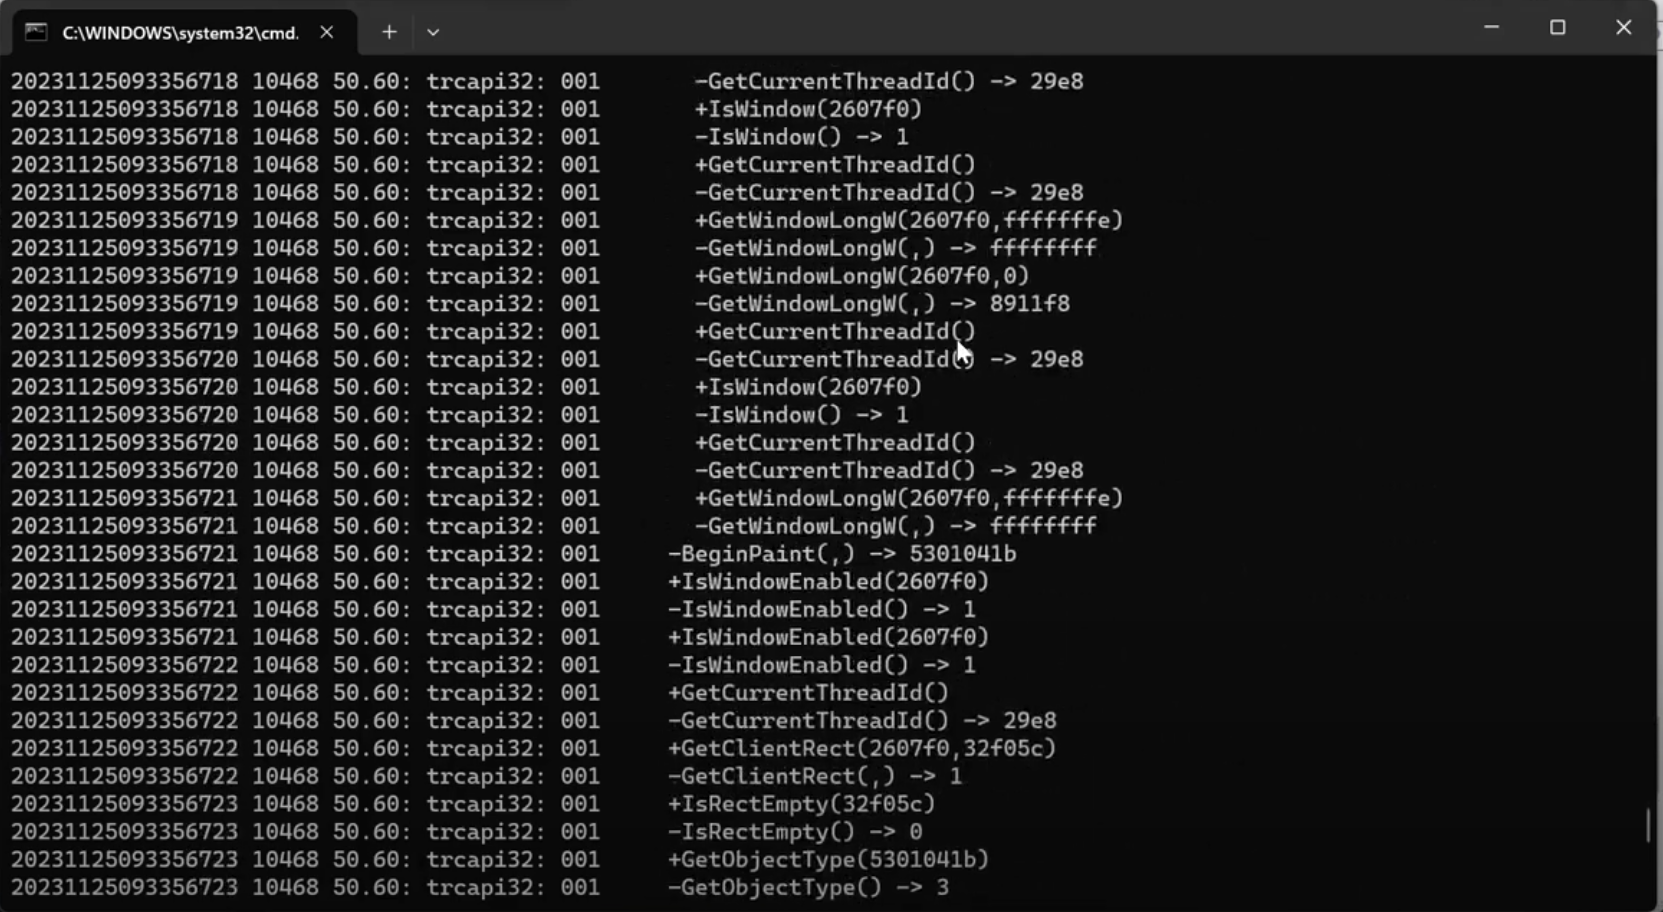
\includegraphics[width=1\textwidth]{./stato-dell-arte/imgs/api_call_example.png}
      \caption{API Call catturate}
      \label{fig:api_call_example}
\end{figure}

Tuttavia, il semplice elenco delle chiamate API non è sufficiente per mostrare la vera natura di un software.\
É necessario definire una logica di analisi che trasformi queste sequenze in informazioni discriminanti. In questa tesi\
tali logiche sono implementate tramite \textit{machine learning}.

\section{Machine Learning}

Il \textit{machine learning} (ML) è una branca dell'intelligenza artificiale (IA) che consente a computer e macchine di apprendere dai dati,\
imitando i processi cognitivi umani\mycite{ibm_machine_learning_2025}.\
In termini pratici, il ML consiste nell'\textbf{addestramento} di un software, detto \textbf{modello},\
per svolgere compiti specifici come effettuare \textbf{previsioni} o generare contenuti (testo, immagini, audio o video)\
a partire da dati osservati\mycite{google_ml_intro}.\
\
Un modello di \textit{machine learning} può essere visto come un costrutto matematico che riceve dati in ingresso (\textit{input})\
e produce un risultato (\textit{output}), in modo analogo a una funzione matematica\mycite{google_ml_glossary_modello}.\
L'\textbf{allenamento} di un modello consiste nel processo di identificazione dei parametri ottimali interni,\
così che il modello possa compiere previsioni accurate; ciò avviene fornendogli una serie di esempi\mycite{google_ml_glossary_allenamento}.\
\
Un \textbf{esempio} è un'istanza di input descritta da un insieme di variabili organizzate in un \textbf{vettore delle caratteristiche}
(\textit{feature vector})\mycite{google_ml_glossary_esempio}.\
Ogni variabile è detta \textbf{caratteristica} (\textit{feature}) e rappresenta un'informazione specifica del dominio del problema\mycite{google_ml_glossary_caratteristica}.\
Le caratteristiche possono essere di tipo \textbf{numerico}, quando esprimono valori quantitativi,\
oppure \textbf{categorico}, quando descrivono attributi qualitativi.\
Una lista di esempi costituisce un \textit{dataset}.

I modelli di \textit{machine learning}, in base al tipo di addestramento e ai dati disponibili,\
possono essere suddivisi in quattro categorie principali:

\begin{itemize}
      \item \textbf{Apprendimento supervisionato}: il modello impara a fare previsioni a partire da dati etichettati,\
            ossia accompagnati dalle risposte corrette, scoprendo le relazioni tra input e output\mycite{google_ml_intro}.
      \item \textbf{Apprendimento non supervisionato}: il modello lavora con dati privi di etichette e ha come obiettivo l'identificazione di strutture o pattern nascosti nei dati\mycite{google_ml_intro}.
      \item \textbf{Apprendimento per rinforzo}: il modello interagisce con un ambiente, ricevendo feedback sotto forma di ricompense o penalità,\
            e sviluppa progressivamente una strategia ottimale per il raggiungimento di un obiettivo\mycite{google_ml_intro}.
      \item \textbf{Apprendimento generativo}: i modelli non si limitano a classificare o predire, ma generano nuovi contenuti (testo, immagini, audio, ecc.)\
            a partire dagli input forniti dall'utente\mycite{google_ml_intro}.
\end{itemize}

In questa tesi ci concentreremo sull'\textbf{apprendimento supervisionato}, affrontando in particolare il compito di \textbf{classificazione}.

\section{Classificazione}

Il compito di \textbf{classificazione} rientra tra quelli affrontabili tramite \textit{apprendimento supervisionato}.\
In questo paradigma, gli esempi utilizzati durante l'addestramento sono accompagnati dall'output corretto, detto\
\textbf{etichetta} (label)\mycite{google_ml_glossary_etichetta}. Nel caso specifico della classificazione, l'etichetta\
corrisponde a una \textbf{classe}, ossia il valore discreto che identifica a quale categoria appartiene l'esempio.\
Allenando quindi un modello su un dataset etichettato, l'obiettivo della classificazione è predire la classe corretta\
di un nuovo esempio non etichettato.

Esistono molteplici compiti di classificazione, distinti uno dall'altro dal numero delle classi da distinguere e da quanto sono\
mutualmente esclusivi\mycite{Belcic_2025}.

\begin{itemize}
      \item \textbf{Classificazione binaria}: le classi tra cui predire sono due e mutualmente esclusive\mycite{Belcic_2025}.
      \item \textbf{Classificazione multi classe}: le classi tra cui predire sono più di due e mutualmente esclusive\mycite{Belcic_2025}.
      \item \textbf{Classificazione a multipla etichetta}: un esempio può appartenere a più classi\mycite{Belcic_2025}.
      \item \textbf{Classificazione non bilanciata}: la distribuzione delle classi di esempio non è equa\mycite{Belcic_2025}.
\end{itemize}

In questo lavoro di tesi verrà affrontata la classificazione multi classe.

\subsection{Algoritmi di Classificazione}

Esistono molteplici algoritmi per la classificazione, in questa tesi verranno affrontanti \textit{XGboost} e \textit{Random forest}.

\subsubsection{Random forest}

Prima di introdurre l'algoritmo di apprendimento \textit{random forest}, è utile esaminare due concetti
fondamentali alla sua comprensione: \textit{bagging} e \textit{decision tree}.

L'algoritmo di apprendimento \textit{bagging} appartiene alla categoria dei metodi di\
\textbf{apprendimento d'insieme}, il cui obiettivo è ridurre la varianza\footnote{La varianza si riferisce\
      alla sensibilità del modello rispetto alle fluttuazioni nei dati di addestramento\mycite{Mucci_2025}.}\
all'interno di un dataset rumoroso\mycite{Bagging_2025}.\
L'apprendimento d'insieme si basa sull'idea che un gruppo di modelli che collaborano possa raggiungere\
prestazioni superiori rispetto a un singolo modello. Questo principio viene spesso associato al concetto\
di ``saggezza delle folle'', secondo cui un insieme di persone fornisce mediamente decisioni migliori di\
quelle di un singolo esperto\mycite{Bagging_2025}.\
Nel \textit{bagging}, i singoli modelli dell'insieme vengono addestrati --- anche in parallelo --- su\
sottoinsiemi del dataset originario, generati tramite campionamento con reinserimento (bootstrap)\mycite{Mucci_2025}.\
Ciò implica che uno stesso esempio possa comparire più volte all'interno di uno o più sottoinsiemi.\
Al termine dell'addestramento, la previsione finale del sistema viene ottenuta aggregando le risposte di\
tutti i modelli. Nel caso della classificazione, la classe predetta corrisponde a quella che ha ricevuto\
il maggior numero di voti.

L'algoritmo \textit{decision tree} è costituito da una serie di domande organizzate gerarchicamente\
a forma di albero. Le domande sono generalmente chiamate \textit{condizioni}, \textit{split} o \textit{test}.\
Ogni nodo interno (non foglia) contiene una condizione, mentre ogni nodo foglia rappresenta una previsione.\
Per effettuare una predizione, si parte dal nodo radice e si percorre l'albero fino a raggiungere un nodo\
foglia, scegliendo il ramo da seguire in base all'esito della condizione presente in ciascun nodo.\
Il percorso che va dalla radice fino alla foglia è chiamato \textit{percorso di inferenza}\mycite{Alberi_decisionali}.

L'algoritmo \textit{Random Forest} è un'estensione dell'algoritmo di \textit{bagging}, in cui i modelli\
interni sono costituiti da \textit{decision tree}. Oltre a essere addestrati su sottoinsiemi casuali degli\
esempi del dataset (\textit{bagging}), ad ogni nodo viene selezionato un sottoinsieme casuale di\
\textit{feature} candidate per effettuare lo \textit{split}. Questo introduce diversità tra gli alberi,\
riducendo la correlazione tra di essi e aumentando la robustezza del modello complessivo\mycite{CheCosEForestaCasuale_2025}.

\subsubsection{XGBoost}

Per una corretta comprensione dell'algoritmo di apprendimento \textit{XGBoost}, è utile\
introdurre preliminarmente l'algoritmo di apprendimento \textit{boosting} e il concetto\
di \textit{ascesa del gradiente}.

Il \textit{boosting} è una tecnica di apprendimento sequenziale in cui più modelli\
vengono addestrati uno dopo l'altro, ciascuno dei quali cerca di correggere gli errori\
commessi dal modello precedente, al fine di ottenere una previsione progressivamente più\
accurata\mycite{CheCoseBoosting_2024}. Il \textit{boosting} appartiene alla categoria degli apprendimenti d'insieme.

La \textit{discesa del gradiente}\mycite{GradientDescent_2025} è un algoritmo di ottimizzazione che permette di trovare i valori ottimali dei
parametri di un modello minimizzando una funzione di costo.
L'idea di base è semplice: si parte da valori iniziali arbitrari per i parametri, si calcola la pendenza (il\
\textit{gradiente}) della funzione di costo in quel punto e si aggiornano i parametri muovendosi nella direzione\
opposta al gradiente, cioè verso la discesa più ripida. Il processo si ripete finché non si raggiunge un minimo\
(locale o globale).\
Un ruolo cruciale è svolto dal \textit{tasso di apprendimento} (\textit{learning rate}), che stabilisce la grandezza\
dei passi: se troppo grande vi è il rischio di superare il minimo, mentre se troppo piccolo l'addestramento\
risulta molto lento. Esistono diverse varianti:\
\begin{itemize}
      \item \textbf{Batch Gradient Descent}: aggiorna i parametri dopo aver visto tutti i dati di addestramento\mycite{GradientDescent_2025}.
      \item \textbf{Stochastic Gradient Descent (SGD)}: aggiorna i parametri dopo ogni esempio, introducendo rumore\
            ma anche la possibilità di sfuggire ai minimi locali\mycite{GradientDescent_2025}.
      \item \textbf{Mini-batch Gradient Descent}: compromesso tra i due, suddivide i dati in piccoli blocchi\mycite{GradientDescent_2025}.
\end{itemize}

L'obiettivo della discesa del gradiente è ridurre progressivamente l'errore, fino a convergere a un set di
parametri che rende il modello il più accurato possibile.

L'algoritmo di apprendimento \textit{XGBoost} si basa sulla tecnica del \textit{boosting}, in cui\
un modello iniziale, l'albero decisionale, viene progressivamente migliorato\
tramite l'uso della \textit{discesa del gradiente}\mycite{KavlakogluRussi_2025}.

\section{Metriche di valutazione}

Per valutare l'efficacia di un classificatore è necessario quantificare quanto esso sia capace di effettuare previsioni corrette.\
Uno strumento utile a questo scopo è la \textbf{matrice di confusione}\mycite{MurelKavlakoglu_2025}.\
\
Nella matrice, le righe rappresentano i valori effettivi mentre le colonne indicano quelli predetti;\
in letteratura è possibile incontrare anche la rappresentazione inversa.\
La matrice ha tante righe e colonne quante sono le classi presenti nel dataset.\
L'intersezione tra la riga $i$ e la colonna $j$ fornisce il numero di istanze della classe\
$i$ che sono state classificate come classe $j$. In particolare, gli elementi della diagonale\
rappresentano le istanze correttamente predette.\
\
A partire dalla matrice di confusione è possibile calcolare diverse metriche di valutazione,\
tra cui la \textbf{precision}, la \textbf{recall} e l'\textbf{F1-score} per ciascuna classe.\
È inoltre possibile derivare le corrispondenti misure aggregate a livello \textit{macro} e\
\textit{micro}, utili per valutazioni globali sul dataset.\
Prima di entrare nel dettaglio delle metriche tornano utili i concetti di \textbf{true positive},\
\textbf{true negative}, \textbf{false positive} e \textbf{false negative} considerando la matrice di confusione $M$ avente $n$ classi.

I \textbf{true positive} di una classe $k$ equivalgono al numero di istanze di classe $k$ che
sono state predette come classe $k$:
\[
      TP_{k} = M_{k,k}
\]

I \textbf{false positive} di una classe $k$ rappresentano il numero di istanze appartenenti a
classi diverse da $k$ che sono state erroneamente predette come $k$:
\[
      FN_{k} = \sum_{\substack{j=1 \\ j \neq k}}^{n} M_{k,j}
\]

I \textbf{false negative} di una classe $k$ rappresentano il numero di istanze appartenenti a
$k$ che sono state erroneamente classificate come un'altra classe:
\[
      FN_{k} = \sum_{\substack{j=1 \\ j \neq k}}^{n} M_{k,j}
\]

I \textbf{true negative} di una classe $k$ rappresentano il numero di istanze appartenenti a
classi diverse da $k$ che sono state correttamente classificate come non $k$:
\[
      TN_{k} = \sum_{\substack{i=1 \\ i \neq k}}^{n}
      \sum_{\substack{j=1 \\ j \neq k}}^{n} M_{i,j}
\]

La \textbf{precision} di una classe $k$ è il rapporto tra i veri positivi e la
somma dei veri positivi e dei falsi positivi:
\[
      \mathrm{Precision}_k = \frac{TP_k}{TP_k + FP_k}
\]

La \textbf{recall} (o sensibilità) di una classe $k$ è il rapporto tra i veri
positivi e la somma dei veri positivi e dei falsi negativi:
\[
      \mathrm{Recall}_k = \frac{TP_k}{TP_k + FN_k}
\]

L'\textbf{F1-score} di una classe $k$ è la media armonica tra precision e recall:
\[
      \mathrm{F1}_k = 2 \cdot \frac{\mathrm{Precision}_k \cdot \mathrm{Recall}_k}
      {\mathrm{Precision}_k + \mathrm{Recall}_k}
\]

Le metriche \textbf{Precision}, \textbf{Recall} e \textbf{F1-Score} calcolate per ciascuna classe
possono essere aggregate per ottenere valori complessivi sul modello intero. Due approcci
comuni di aggregazione sono la media \textit{macro} e la media \textit{micro}:

\[
      \mathrm{Macro_{precision}} = \frac{\sum_{i}^{n} Precision_{i}}{n}
\]

\[
      \mathrm{Macro_{recall}} = \frac{\sum_{i}^{n} Recall{i}}{n}
\]

\[
      \mathrm{Macro_{F1}} = \frac{\sum_{i}^{n} F1{i}}{n}
\]

\[
      \mathrm{Micro_{Precision}} = \frac{\sum_{i}^{n} TP_{i}}{\sum_{i}^{n} TP_{i} + \sum_{i}^{n} FP_{i}}
\]

\[
      \mathrm{Micro_{Recall}} = \frac{\sum_{i}^{n} TP_{i}}{\sum_{i}^{n} TP_{i} + \sum_{i}^{n} FN_{i}}
\]

\[
      \begin{aligned}
            TP               & = \sum_{i=1}^{n} TP_i,                                                                  & FP            & = \sum_{i=1}^{n} FP_i, & FN & = \sum_{i=1}^{n} FN_i, \\[1mm]
            \text{Precision} & = \frac{TP}{TP + FP},                                                                   & \text{Recall} & = \frac{TP}{TP + FN},                                \\[1mm]
            \text{Micro-F1}  & = 2 \cdot \frac{\text{Precision} \cdot \text{Recall}}{\text{Precision} + \text{Recall}}
      \end{aligned}
\]

\section{Approcci di Machine Learning per Windows PE Malware Detection}

Diversi studi hanno affrontato il problema della rilevazione dei malware in ambiente Windows
basandosi sull'analisi delle chiamate API.

Ad esempio, Zhang et al. (2015) propongono un approccio innovativo per la rilevazione di malware basato sull'analisi dinamica delle sequenze di chiamate API.\
Gli autori applicano algoritmi di allineamento delle sequenze di DNA per identificare somiglianze tra le sequenze di chiamate API\
di programmi legittimi e malware.\
Questa metodologia consente di rilevare comportamenti malevoli anche in presenza di tecniche di offuscamento.\
Il modello proposto ha mostrato buone prestazioni nella classificazione dei malware, evidenziando l'efficacia dell'approccio basato sull'allineamento\
delle sequenze di chiamate API\mycite{KiKim_2015}.

Amer e Zelinka (2020) propongono un approccio basato sulla modellazione semantica delle sequenze di API.\
Le chiamate vengono rappresentate come vettori tramite \textit{Word2Vec}, raggruppate mediante \textit{clustering}\
e poi modellate con catene di Markov, ottenendo matrici di transizione distinte per malware e software legittimo.\
Il modello raggiunge un'accuratezza di rilevamento fino al 99\% e permette previsioni precoci già dalle prime chiamate API\mycite{Amer_Zelinka_2020}.

Un contributo più recente è quello di Gond e Mohapatra (2025), che affrontano la classificazione dei
malware dinamici considerando il fenomeno del \textit{concept drift}, ovvero la variazione dei comportamenti
dei malware nel tempo. Gli autori combinano tecniche di deep learning con meccanismi di adattamento al drift:
le sequenze di API raccolte tramite sandbox vengono trasformate in rappresentazioni linguistiche
tramite n-grammi e filtrate per rilevanza. Successivamente, un algoritmo genetico genera varianti delle
feature per simulare nuovi schemi comportamentali emergenti. La classificazione è affidata a reti neurali
artificiali, ricorrenti e convoluzionali (CNN), raggiungendo accuratezze fino al 99,5\% anche in presenza
di mutazioni nei dati. L'integrazione del genetic algorithm consente di ridurre la perdita di performance
dovuta al concept drift\mycite{Gond_Mohapatra_2025}.

Questi studi evidenziano come l'analisi delle sequenze di API, se combinata con tecniche di
rappresentazione avanzata e modelli adattativi, possa migliorare sensibilmente l'efficacia della
malware detection in ambienti Windows.

%-------------------------------------------------------------------------------
% BIBLIOGRAFIA
%-------------------------------------------------------------------------------
\bibliographystyle{IEEEtran}
\bibliography{bibliografia}


%-------------------------------------------------------------------------------
% PARTI FINALI DEL DOCUMENTO
%-------------------------------------------------------------------------------
%\cleardoublepage
%\chapter*{Ringraziamenti}

\newpage
\null
\newpage

\newpage
\null
\newpage

\newpage
\null
\newpage

\end{document}